% This file was created by matlab2tikz.
%
\definecolor{mycolor1}{rgb}{0.89412,0.10196,0.10980}%
\definecolor{mycolor2}{rgb}{0.21569,0.49412,0.72157}%
%
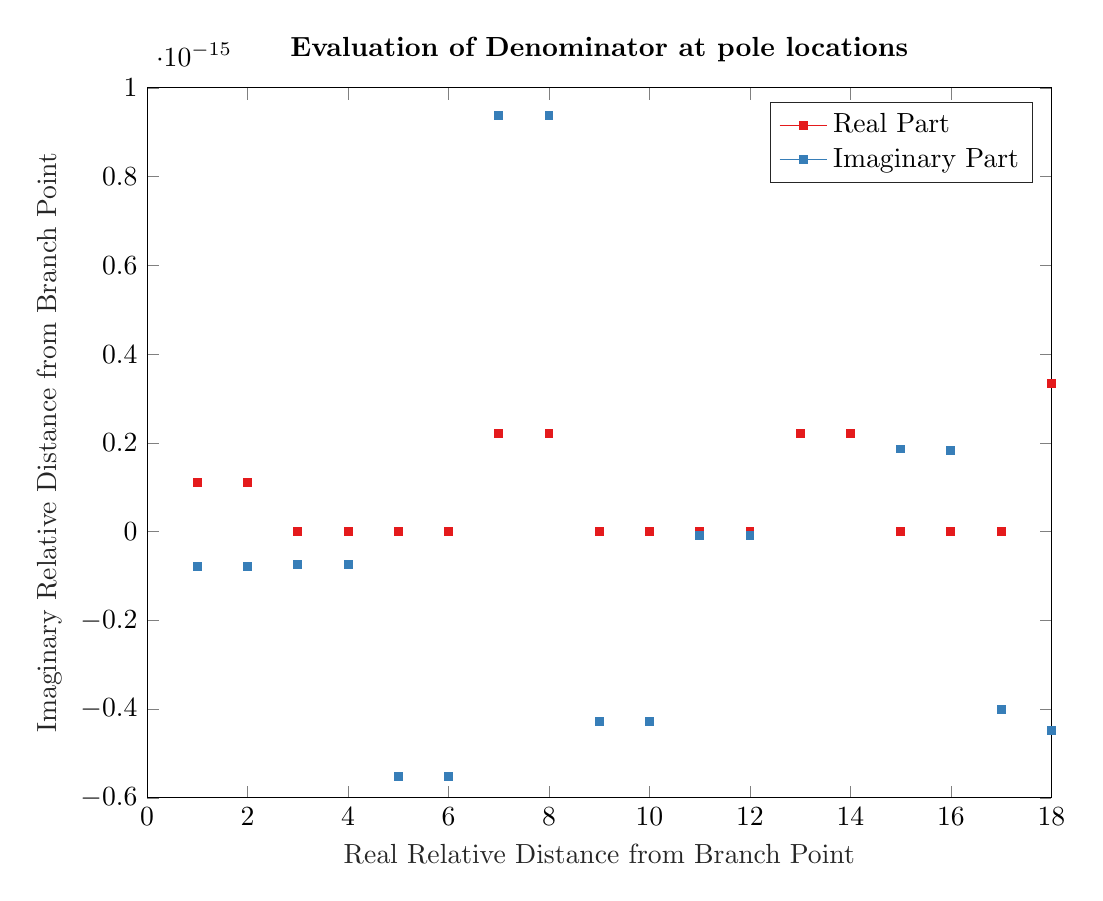
\begin{tikzpicture}

\begin{axis}[%
width=4.521in,
height=3.55in,
at={(0.758in,0.497in)},
scale only axis,
xmin=0,
xmax=18,
xlabel style={font=\color{white!15!black}},
xlabel={$\textrm{Real Relative Distance from Branch Point}$},
ymin=-6e-16,
ymax=1e-15,
ylabel style={font=\color{white!15!black}},
ylabel={$\textrm{Imaginary Relative Distance from Branch Point}$},
axis background/.style={fill=white},
title style={font=\bfseries},
title={Evaluation of Denominator at pole locations},
legend style={legend cell align=left, align=left, draw=white!15!black}
]
\addplot [color=mycolor1, draw=none, mark size=1.4pt, mark=square*, mark options={solid, fill=mycolor1, mycolor1}]
  table[row sep=crcr]{%
1	1.11022302462516e-16\\
2	1.11022302462516e-16\\
3	0\\
4	0\\
5	0\\
6	0\\
7	2.22044604925031e-16\\
8	2.22044604925031e-16\\
9	0\\
10	0\\
11	0\\
12	0\\
13	2.22044604925031e-16\\
14	2.22044604925031e-16\\
15	0\\
16	0\\
17	0\\
18	3.33066907387547e-16\\
};
\addlegendentry{Real Part}

\addplot [color=mycolor2, draw=none, mark size=1.4pt, mark=square*, mark options={solid, fill=mycolor2, mycolor2}]
  table[row sep=crcr]{%
1	-7.84420271793262e-17\\
2	-7.84420271793262e-17\\
3	-7.45795569398466e-17\\
4	-7.45795569398466e-17\\
5	-5.51065235923544e-16\\
6	-5.51065235923544e-16\\
7	9.37299395558619e-16\\
8	9.37299395558619e-16\\
9	-4.27599900351855e-16\\
10	-4.27599900351855e-16\\
11	-9.41963503073336e-18\\
12	-9.41963503073336e-18\\
13	8.75889522185524e-16\\
14	8.75889522185524e-16\\
15	1.8606708935351e-16\\
16	1.83427642872817e-16\\
17	-4.00020706732987e-16\\
18	-4.47586108354532e-16\\
};
\addlegendentry{Imaginary Part}

\end{axis}
\end{tikzpicture}%